\chapter{Etalon}\label{etalon}
	\section{Introduction}
The etalon is an optical device made of two perfectly parallel semi-reflecting surfaces. It can be thought as a Fabry-P\'erot cavity which walls are fixed. This geometry can be implemented either with an air-based or a solid design. The first one consists in two surfaces separated by air, one of which usually can be moved via piezoelectric actuators. The second one is just made from a piece of glass (or other materials suitable for the desired application) with a partially reflecting coating covered facets (\cref{solidstate}). While the air based etalons make longer cavities, thus more precise, they are extremely delicate and cumbersome to manage, mostly because the two surfaces must be kept parallel within hundredths of wavelength. The solid state ones, on the other hand, are usually smaller and less performing, but way more robust and easier to use.

Every time the impinging beam encounters one of the two optical surfaces the light is partially reflected and partially transmitted. Multiple reflections occur inside the two surfaces leading to an infinite number of rays departing from the interferometer in both the transmitted and reflected directions. Contiguous beams differ for a constant phase and this causes an interference pattern, as shown in \cref{etalonmonitor}.

\begin{figure}[!hbt]\centering
\begin{minipage}[t]{0.46\textwidth}\centering
\includegraphics[width=\linewidth, height=5cm, draft=\foto]{eps/etalon5.eps}
\caption{Solid state etalons.}
\label{solidstate}
\end{minipage}
\hfill
\begin{minipage}[t]{0.46\textwidth}\centering
\includegraphics[width=\linewidth, height=5cm, draft=\foto]{eps/thering.eps}
\caption{The etalon diffraction pattern seen through our video camera.}
\label{etalonmonitor}
\end{minipage}
\end{figure}

	\section{Theoretical treatment}
To derive the phase difference between two adjacent beams, let's begin calculating the difference in their optical paths (\cref{fig:angoli}). We thus choose two parallel beams, such as $OB$ and $CD$, and draw a wavefront perpendicular to them, $AC$. 
\begin{figure}[!htb]\centering
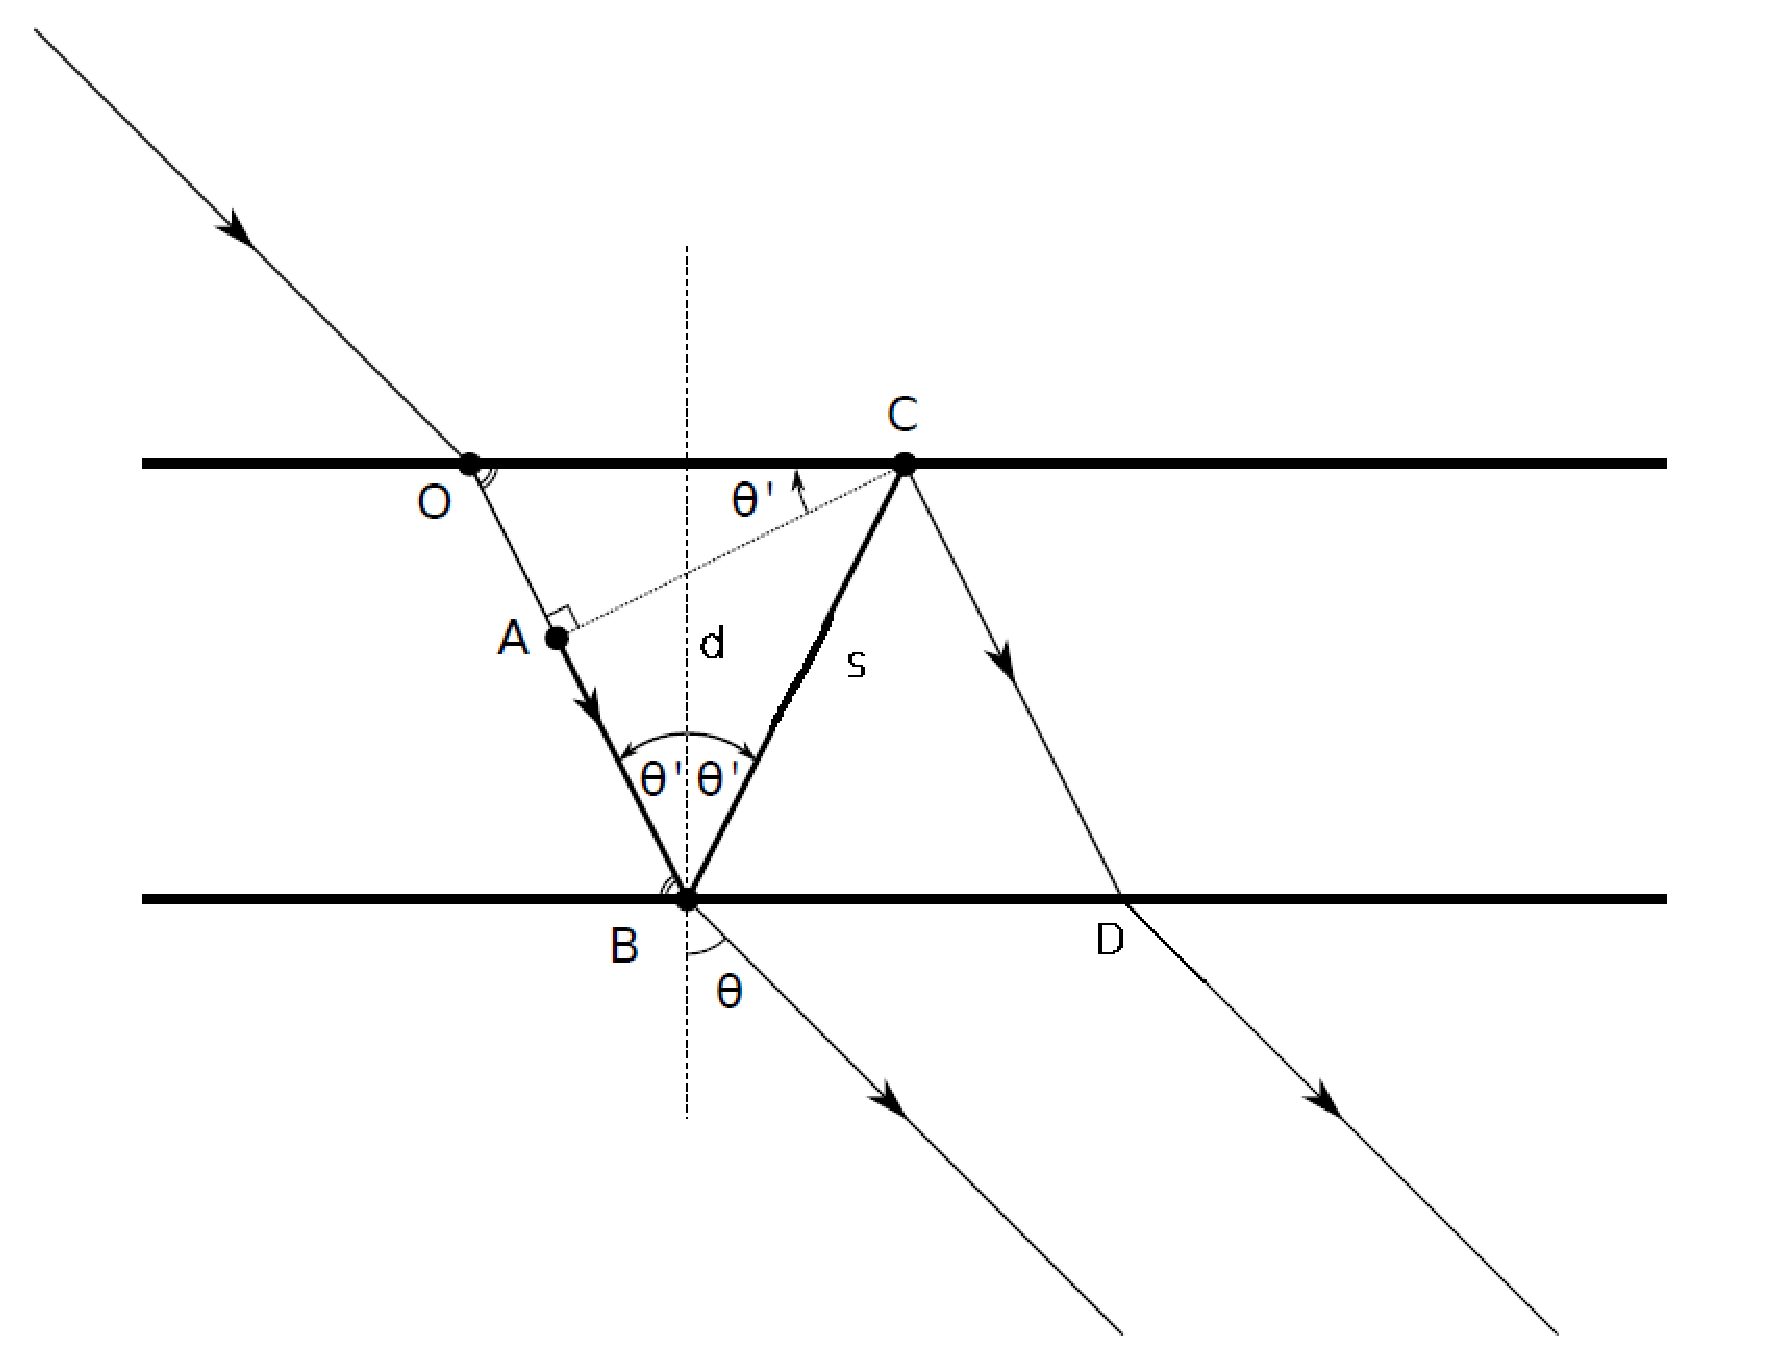
\includegraphics[width=.8\linewidth, draft=\foto]{eps/angoli.eps}
\caption{The impinging beam changes direction due to refraction index difference between the air and the medium, the angles $\theta$ and $\theta'$ being related to the refraction indices $n$ (air) and $n'$ (medium) by Snell's law.}
\label{fig:angoli}
\end{figure}
The optical path difference between $A$ and $C$ is given by
\mate
\overline{ABC}=\overline{AB}+\overline{BC}
\atem
 We call $d$ the width of the etalon, and $s$ the distance traveled by the beam from one surface to the other one, so that
\mate
\overline{BC}=\overline{OB}\equiv s=\frac{d}{\cos\theta'}.
\atem
From elementary geometry considerations we get the following relationships:
\begin{align}
\overline{AB}&=\overline{OB}-\overline{OA}\\
\overline{OA}&=\sqrt{\overline{OC}^2-\overline{AC}^2}\\
\overline{OC}&=2s\sin\theta'\\
\overline{AC}&=s\sin(2\theta')
\end{align}
Then we write
\begin{align}
\overline{OA}&=\sqrt{4s^2\sin^2\theta'-s^2\sin^2(2\theta')}
\nona \sqrt{4s^2\sin^2\theta'\left(1-\frac{\sin^2(2\theta')}{4\sin^2\theta'}\right)}
\nona 2s\sin\theta'\sqrt{1-\cos^2\theta'}
\nona 2s\sin^2\theta'
\end{align}
Putting all together we get the optical path difference

\begin{align}
\overline{ABC}&=\overline{AB}+\overline{BC}
\nona \overline{OB}-\overline{OA}+\overline{BC}
\nona s-2s\sin^2\theta'+s
\nona2s(1-\sin^2\theta')
\nona2s\cos^2\theta'
\nona2d\cos\theta'.
\end{align}

If the incident light has wavelength $\lambda_0$ in the vacuum and the etalon medium has refractive index $n'$, the light wave vector inside the medium is
\mate
k=\frac{2\pi}{\lambda_0}n'
\atem
and the phase shift between two adjacent rays is 
\mate
\Delta=k\cdot\overline{ABC}=\frac{4\pi}{\lambda_0}n'd\cos\theta'
\label{phase}
\atem

Now, indicating by $T$ the overall etalon transmission coefficient and by $R$ the reflection coefficient correspondig to one round-trip, the total amplitude of the electric field in some point after the etalon is the sum of those of the subsequent rays
\mate
E_{\mai{T}}=E_{\mai{0}}T+E_{\mai{0}}TRe^{i\Delta}+E_{\mai{0}}TR^2e^{i2\Delta}+E_{\mai{0}}TR^3e^{i3\Delta}+\dots
\atem
which is nothing but the geometrical series, that can be summed up ($|Re^{i\Delta}|<1$) to yield 
\mate
E_{\mai{T}}=E_{\mai{0}}T\sum_{j}\left(Re^{i\Delta}\right)^j=\frac{E_{\mai{0}}T}{1-Re^{i\Delta}}
\atem

What we observe is actually the transmitted intensity 

\mate
I_{\mai{T}}=|E_{\mai{T}}|^2=|E_{\mai{0}}|^2\frac{T^2}{|1-Re^{i\Delta}|^2}
\atem

The denominator can be rewritten as
\begin{align}
|1-Re^{i\Delta}|&=(1-Re^{i\Delta})(1-Re^{-i\Delta})
\nona 1-R(e^{i\Delta}+e^{-i\Delta})+R^2
\nona 1-2R\cos\Delta+R^2
\nona 1-2R\left(1-2\sin^2\frac{\Delta}{2}\right)+R^2
\nona 1-2R+4R\sin^2\frac{\Delta}{2}+R^2
\nona \nonumber (1-R)^2+4R\sin^2\frac{\Delta}{2}\\
&= (1-R)^2\left(1+\frac{4R}{(1-R)^2}\sin^2\frac{\Delta}{2}\right)
\end{align}

So that the transmitted intensity becomes
\mate
I_{\mai{T}}=I_{\mai{0}}\frac{T^2}{(1-R)^2}\frac{1}{\left(1+\frac{4R}{(1-R)^2}\sin^2\frac{\Delta}{2}\right)}
\label{intensity}
\atem

One defines a \textit{peak constant}
\mate
C_{\mai{peak}}\equiv\frac{T^2}{(1-R)^2}
\atem

which is equal to 1 for an ideal surface such that $1=R+T$. In a real surface, instead, some absorption $A$ is present, so that $1=R+T+A$. The peak constant in this case can be rewritten as
\mate
C_{\mai{peak}}=\frac{(1-A-R)^2}{(1-R)^2}=\left(1-\frac{A}{1-R}\right)^2
\atem 

Furthermore we shall define the \textit{coefficient of finesse}\footnote{Not to be confused with the \textit{finesse} defined further in this discussion (pg.~\pageref{finesse}). These parameters are strongly correlated, though, and literature is not uniform on which of them is to be called \textquotedblleft finesse\textquotedblright.}
\mate
F\equiv\frac{4R}{(1-R)^2}.
\atem

In the ideal etalon case we have $A\simeq0$, which implies $C_{\mbox{peak}}\simeq1$,  so that \cref{intensity} eventually reduces to
\mate
I_{\mai{T}}=I_{\mai{0}}\ \frac{1}{1+F\sin^2\frac{\Delta}{2}}
\atem

The transmitted intensity is thus given by the constant input intensity value, modulated by the so called \textit{Airy function} plotted in \cref{Airyplot}
\mate
\frac{I_{\mai{T}}}{I_{\mai{0}}}=\frac{1}{1+F\sin^2\frac{\Delta}{2}}\equiv A[F;\Delta]
\atem

\begin{figure}[!htb]\centering
% GNUPLOT: LaTeX picture with Postscript
\begingroup
  \makeatletter
  \providecommand\color[2][]{%
    \GenericError{(gnuplot) \space\space\space\@spaces}{%
      Package color not loaded in conjunction with
      terminal option `colourtext'%
    }{See the gnuplot documentation for explanation.%
    }{Either use 'blacktext' in gnuplot or load the package
      color.sty in LaTeX.}%
    \renewcommand\color[2][]{}%
  }%
  \providecommand\includegraphics[2][]{%
    \GenericError{(gnuplot) \space\space\space\@spaces}{%
      Package graphicx or graphics not loaded%
    }{See the gnuplot documentation for explanation.%
    }{The gnuplot epslatex terminal needs graphicx.sty or graphics.sty.}%
    \renewcommand\includegraphics[2][]{}%
  }%
  \providecommand\rotatebox[2]{#2}%
  \@ifundefined{ifGPcolor}{%
    \newif\ifGPcolor
    \GPcolorfalse
  }{}%
  \@ifundefined{ifGPblacktext}{%
    \newif\ifGPblacktext
    \GPblacktexttrue
  }{}%
  % define a \g@addto@macro without @ in the name:
  \let\gplgaddtomacro\g@addto@macro
  % define empty templates for all commands taking text:
  \gdef\gplbacktext{}%
  \gdef\gplfronttext{}%
  \makeatother
  \ifGPblacktext
    % no textcolor at all
    \def\colorrgb#1{}%
    \def\colorgray#1{}%
  \else
    % gray or color?
    \ifGPcolor
      \def\colorrgb#1{\color[rgb]{#1}}%
      \def\colorgray#1{\color[gray]{#1}}%
      \expandafter\def\csname LTw\endcsname{\color{white}}%
      \expandafter\def\csname LTb\endcsname{\color{black}}%
      \expandafter\def\csname LTa\endcsname{\color{black}}%
      \expandafter\def\csname LT0\endcsname{\color[rgb]{1,0,0}}%
      \expandafter\def\csname LT1\endcsname{\color[rgb]{0,1,0}}%
      \expandafter\def\csname LT2\endcsname{\color[rgb]{0,0,1}}%
      \expandafter\def\csname LT3\endcsname{\color[rgb]{1,0,1}}%
      \expandafter\def\csname LT4\endcsname{\color[rgb]{0,1,1}}%
      \expandafter\def\csname LT5\endcsname{\color[rgb]{1,1,0}}%
      \expandafter\def\csname LT6\endcsname{\color[rgb]{0,0,0}}%
      \expandafter\def\csname LT7\endcsname{\color[rgb]{1,0.3,0}}%
      \expandafter\def\csname LT8\endcsname{\color[rgb]{0.5,0.5,0.5}}%
    \else
      % gray
      \def\colorrgb#1{\color{black}}%
      \def\colorgray#1{\color[gray]{#1}}%
      \expandafter\def\csname LTw\endcsname{\color{white}}%
      \expandafter\def\csname LTb\endcsname{\color{black}}%
      \expandafter\def\csname LTa\endcsname{\color{black}}%
      \expandafter\def\csname LT0\endcsname{\color{black}}%
      \expandafter\def\csname LT1\endcsname{\color{black}}%
      \expandafter\def\csname LT2\endcsname{\color{black}}%
      \expandafter\def\csname LT3\endcsname{\color{black}}%
      \expandafter\def\csname LT4\endcsname{\color{black}}%
      \expandafter\def\csname LT5\endcsname{\color{black}}%
      \expandafter\def\csname LT6\endcsname{\color{black}}%
      \expandafter\def\csname LT7\endcsname{\color{black}}%
      \expandafter\def\csname LT8\endcsname{\color{black}}%
    \fi
  \fi
  \setlength{\unitlength}{0.0500bp}%
  \begin{picture}(7200.00,5040.00)%
    \gplgaddtomacro\gplbacktext{%
      \csname LTb\endcsname%
      \put(946,704){\makebox(0,0)[r]{\strut{} 0}}%
      \csname LTb\endcsname%
      \put(946,1439){\makebox(0,0)[r]{\strut{} 0.2}}%
      \csname LTb\endcsname%
      \put(946,2174){\makebox(0,0)[r]{\strut{} 0.4}}%
      \csname LTb\endcsname%
      \put(946,2909){\makebox(0,0)[r]{\strut{} 0.6}}%
      \csname LTb\endcsname%
      \put(946,3644){\makebox(0,0)[r]{\strut{} 0.8}}%
      \csname LTb\endcsname%
      \put(946,4379){\makebox(0,0)[r]{\strut{} 1}}%
      \csname LTb\endcsname%
      \put(1078,484){\makebox(0,0){\strut{}$-3\pi$}}%
      \csname LTb\endcsname%
      \put(2032,484){\makebox(0,0){\strut{}$-2\pi$}}%
      \csname LTb\endcsname%
      \put(2986,484){\makebox(0,0){\strut{}$-\pi$}}%
      \csname LTb\endcsname%
      \put(3941,484){\makebox(0,0){\strut{}$0$}}%
      \csname LTb\endcsname%
      \put(4895,484){\makebox(0,0){\strut{}$\pi$}}%
      \csname LTb\endcsname%
      \put(5849,484){\makebox(0,0){\strut{}$2\pi$}}%
      \csname LTb\endcsname%
      \put(6803,484){\makebox(0,0){\strut{}$3\pi$}}%
      \put(176,2541){\rotatebox{-270}{\makebox(0,0){\strut{}$A[F;\Delta]$}}}%
      \put(3940,154){\makebox(0,0){\strut{}Phase shift ($\Delta$)}}%
      \put(3940,4709){\makebox(0,0){\strut{}The Airy function for different values of F}}%
    }%
    \gplgaddtomacro\gplfronttext{%
      \csname LTb\endcsname%
      \put(4336,4232){\makebox(0,0)[l]{\strut{}F = 1}}%
      \csname LTb\endcsname%
      \put(4336,4012){\makebox(0,0)[l]{\strut{}F = 10}}%
      \csname LTb\endcsname%
      \put(4336,3792){\makebox(0,0)[l]{\strut{}F = 100}}%
    }%
    \gplbacktext
    \put(0,0){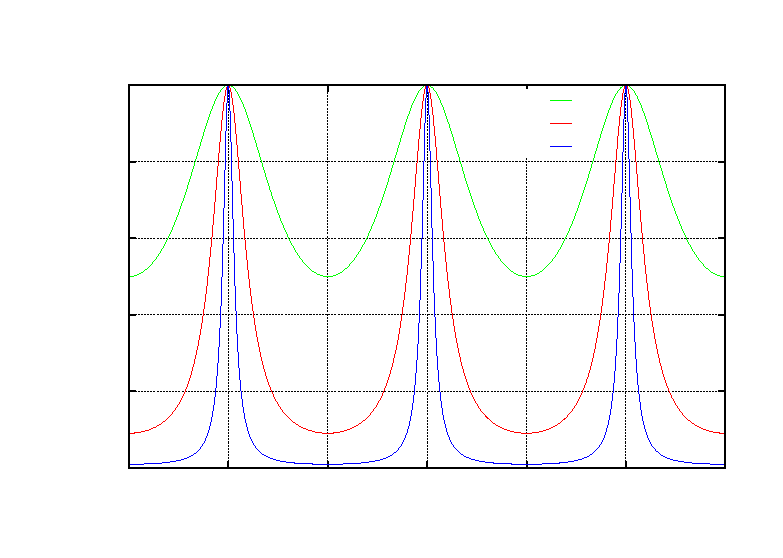
\includegraphics{eps/Airy}}%
    \gplfronttext
  \end{picture}%
\endgroup

\caption{The Airy function peaks when the phase shift is an integer multiple of $2\pi$. As the finesse coefficient increases, the peaks become more sharp and their position is better defined.}
\label{Airyplot}
\end{figure}
	\section{Interference pattern}\label{interferencepattern}
As is clear from \cref{Airyplot}, the interference maxima take place for $\Delta=2m\pi$, where $m$ is an integer representing the order of diffraction.
From \cref{phase} we have
\mate
m=\frac{2n'}{\lambda_0}d\cos\theta'
\label{ordine}
\atem
Looking at \cref{intensity}, we define the intensity at the maximum and at the minimum as
\begin{align}
I_{\mai{max}}&\equiv\frac{I_{\mai{T}}[\Delta=2m\pi]}{I_{\mai{0}}}=C_{\mai{peak}}=\frac{T^2}{(1-R)^2}\\
I_{\mai{min}}&\equiv\frac{I_{\mai{T}}[\Delta=(2m+1)\pi]}{I_{\mai{0}}}=\frac{T^2}{(1-R)^2+4R}=\frac{T^2}{(1+R)^2}
\end{align}
We shall now define a \textit{contrast factor}
\mate
\mathcal{C}\equiv\frac{I_{\mai{max}}}{I_{\mai{min}}}=\left(\frac{1+R}{1-R}\right)^2=1+F
\atem
which is also a useful parameter in the characterization of an etalon.

To describe how defined are the peaks, we have to consider their full width at half maximum (FWHM). Thus we observe the points around a maximum whose intensity is $I_{T}=I_{\mai{max}}/2$. They have a phase shift 
\mate
\Delta=2m\pi\pm\frac{\varepsilon}{2}
\atem

where $\varepsilon$ is now the FWHM expressed as a phase. Putting this into \cref{intensity} we get the identity

$$\frac{1}{2}=\frac{1}{1+F\sin^2\frac{\varepsilon}{4}}\quad;$$ $$F\sin^2\frac{\varepsilon}{4}=1$$

If now we approximate $\sin\left(\varepsilon/4\right)\simeq\varepsilon/4$ we get the phase expression for the FWHM, as a function of the coefficient of finesse $F$
\mate
\varepsilon=\frac{4}{\sqrt{F}}
\atem
Two contiguous maxima are separated by the quantity known as \textit{free spectral range} (FSR). In the frequency domain its value depends on the device, and is actually one of the parameters characterizing an etalon. In the phase domain its value is always $2\pi$, by definition. Doing the ratio between the peaks separation and their width, one gets a very important parameter which is called the \textit{finesse} of the etalon
\mate
\mathcal{F}\equiv\frac{2\pi}{\varepsilon}=\frac{\pi}{2}\sqrt{F}=\frac{\pi\sqrt{R}}{1-R}
\label{finesse}
\atem
	\section{Etalon as a spectroscope}\label{etalonspec}
It is possible to build a direct relationship between the angular separation of the rings and the wavelength $\lambda_0$ of the incident light.
We put ourself under the approximation of nearly perpendicular incident light, so that
$$\sin\theta'\simeq\theta'$$$$\sin\theta\simeq\theta$$
Snell's law then simplifies to
$$\frac{\sin\theta'}{n'}=\frac{\sin\theta}{n}\quad\Rightarrow\quad\frac{\theta'}{n'}=\frac{\theta}{n}$$
The small angles approximation also implies
\begin{align} 
\cos\theta'&\simeq1-\frac{\theta'^2}{2}\nonumber\\
&\simeq1-\left(\frac{n'}{n}\right)^2\frac{\theta^2}{2}\nonumber
\end{align}
These approximations being valid, we recall \cref{ordine}
$$m=\frac{2n'}{\lambda_0}d\cos\theta'\quad\Rightarrow\quad m=\frac{2n'}{\lambda_0}d\left(1-\left(\frac{n'}{n}\right)^2\frac{\theta^2}{2}\right)$$

For a normal incident wave we have

\mate
m_0=\frac{2n'd}{\lambda_0}\equiv m_1+e
\atem
where we defined $m_1$ and $e$ as the integer and fractional part of $m_0$, respectively.

Putting together the above equations we find 

\begin{align}
\theta&=\frac{1}{n}\sqrt{\frac{n'\lambda_0}{d}}\sqrt{\frac{2n'd}{\lambda_0}-m}\nonumber\\
&=\frac{1}{n}\sqrt{\frac{n'\lambda_0}{d}}\sqrt{m_1-m+e}
\end{align}

Now, by redefining the integer part as $m_1-m=p-1$, we obtain the angle for the p\textit{th} order:
\mate
\theta_p=\frac{1}{n}\sqrt{\frac{n'\lambda_0}{d}}\sqrt{p-1+e}
\atem
and if we focus the rings onto a screen with a convergent lens, of focal ratio $f$, the diameter of the bright ring is
\mate
D^2_p=(2f\theta_p)^2=\frac{4n'\lambda_0f^2}{n^2d}(p-1+e).
\atem